
\chapter{SYSTEM DESIGN AND IMPLEMENTATION}
\label{ch:system}
Follow My Voice is a gaze-contingent voice guidance system designed to help a seated user find a target object in a surrounding search scene. The system divides responsibility between a local guidance layer, which owns all spatial reasoning, and a cloud language model agent, Jev, which decides how and when to speak. Figure~\ref{fig:architecture} summarizes the pipeline from sensing to speech output. This division makes spatial eligibility logic deterministic and traceable while allowing the agent to adapt the phrasing and timing of guidance to the user's recent behavior.

\section{Apparatus}
The application is developed in Unity 6 (6000.3.10f1) using the Unity OpenXR Plugin (1.16.1), HTC VIVE OpenXR integration (2.5.1), and Unity XR Interaction Toolkit (3.3.1). It is deployed as a standalone Android ARM64 application on the HTC VIVE Focus Vision head-mounted display, with rendering performed locally on the headset using the Universal Render Pipeline (17.3.0). The headset supplies head-pose and eye-gaze tracking, while the tracked right-hand controller supplies pointing and trigger input. Video passthrough supports the mixed-reality view. Network access supports cloud-based agent decisions and voice preparation; it is not used to stream rendered frames from a host computer.

\section{Search Task}
The search task takes place in mixed reality using video passthrough in a neutral physical room. Participants will sit on a swivel chair and interact using the right controller. Virtual colored geometric objects hang on eight vertical planes anchored along the surrounding walls. Figure~\ref{fig:scene} shows the layout from above. The application holds the target identity, which is withheld from the opening instructions, so participants must rely on voice guidance to locate it. Participants select an object by pointing the controller ray at it and pressing the trigger. Stimulus density and spatial bounds will be frozen for the study release after seated-comfort and ray-selection pilots. For each trial, the system logs object positions, layout seed, wall assignment, and target identity.

\begin{figure}[htbp]\centering
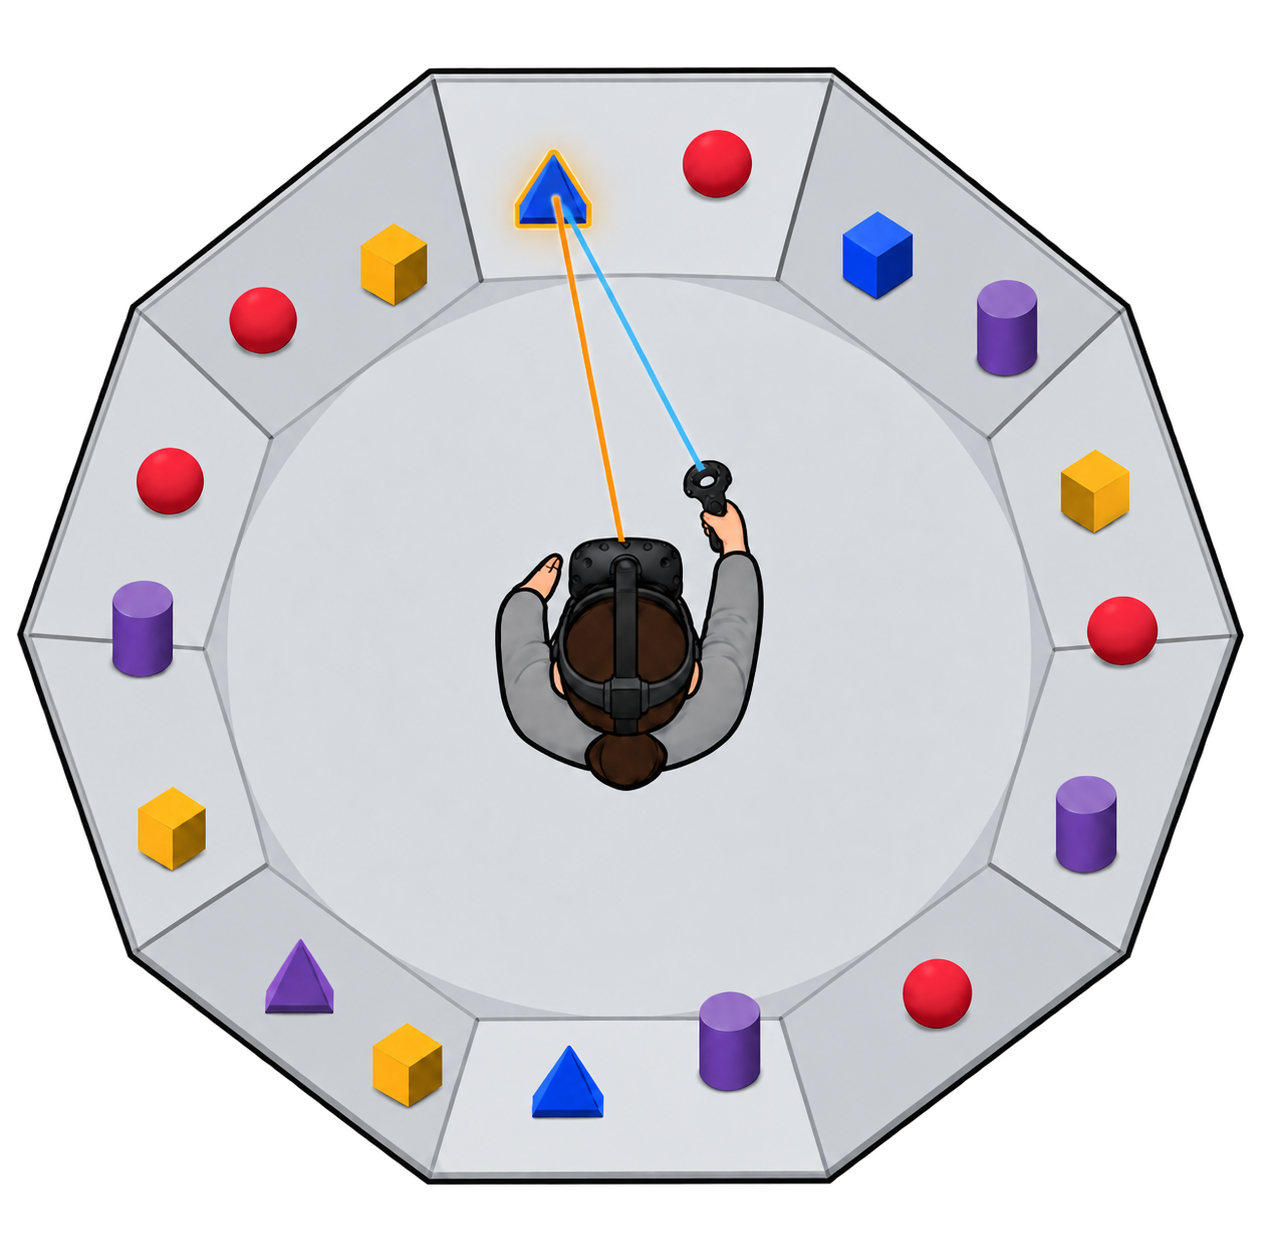
\includegraphics[width=0.70\linewidth,alt={Overhead scene illustration showing a seated headset wearer, surrounding vertical object panels, and gaze and controller rays.}]{figures/image.png}
\caption[Search-scene illustration]{Top-down view of the search scene. The seated participant is surrounded by wall panels holding colored geometric objects. The gaze ray (orange) and controller ray (blue) converge on the highlighted target, the state in which the participant is ready to select with the trigger. The layout is illustrative; the drawn object count is schematic; object positions and target identity vary by trial. The converging rays and highlighted endpoint illustrate interaction, not an advance participant-visible target-identification cue.}
\label{fig:scene}
\end{figure}

\section{Sensing and Guidance State}
The system continuously collects eye-gaze origin, direction, and validity; head pose; right-controller pose; and ray-object intersections. A local state machine combines these observations with the target geometry to track the participant's progress through the search: turning toward the target wall, refining within the wall, acquiring the target with gaze, pointing with the controller, and becoming ready to select. Additional states cover suspended or paused operation. Each state transition is logged with its cause.

Because guidance is only as reliable as the evidence behind it, the state machine issues new gaze-dependent guidance only when gaze data are valid and recent. Gaze ray hits, gaze-vicinity candidates, and controller hits are treated as separate observations. When gaze-vicinity regions overlap, the closest object is chosen as the vicinity candidate. A controller ray hit on the target immediately suppresses contradictory directional cues. The spoken pointing acknowledgment separately requires a one-second controller hold with valid nearby gaze when speech is admitted. Suppression is intended to prevent away-directions during the qualification interval without falsely acknowledging an unqualified hold. Gaze confirmation, controller confirmation, and trigger selection are recorded as distinct events.

\section{Short-Term Interaction Memory}
To give guidance continuity, the system maintains two short-term memories. A spatial history tracks turning progress and supports cues that return the participant to the target. A speech-decision memory records what the system actually said and how the guidance state changed. Each speech entry stores its relative age, context, and whether playback completed or was interrupted; each state entry stores the prior and current states and the reason for the transition. The speech and transition lists each retain at most four entries; snapshots sent to Jev exclude entries older than 15 seconds. This bounded recent context is related to the context-management motivation of EmBARDiment~\cite{bovo2025embardiment}, but the current implementation does not use its object-admission or dropout policy. The separate spatial history retains up to three seconds or 384 target-relative gaze observations and clears on invalid evidence, source changes, or observation gaps longer than 100~ms. These limits are engineering settings, not validated fixation or blink thresholds. Gaze-vicinity confirmation currently requires 100~ms of valid qualifying evidence; invalid evidence resets its entry timer, and reacquisition after a spoken confirmation requires 150~ms of valid gaze away. Those interaction gates do not admit objects to speech memory, and missing gaze is not counted as observed dwell. Both memory types are cleared whenever guidance resets and is copied before each asynchronous request. This memory is deliberately scoped to the current task: it does not build a persistent participant profile or attempt to infer unobserved mental states.

Figure~\ref{fig:bounded-memory} shows which recent evidence accompanies an asynchronous request. Its time limits bound the software context and must not be interpreted as estimates of human short-term memory.

\begin{figure}[htbp]
\centering
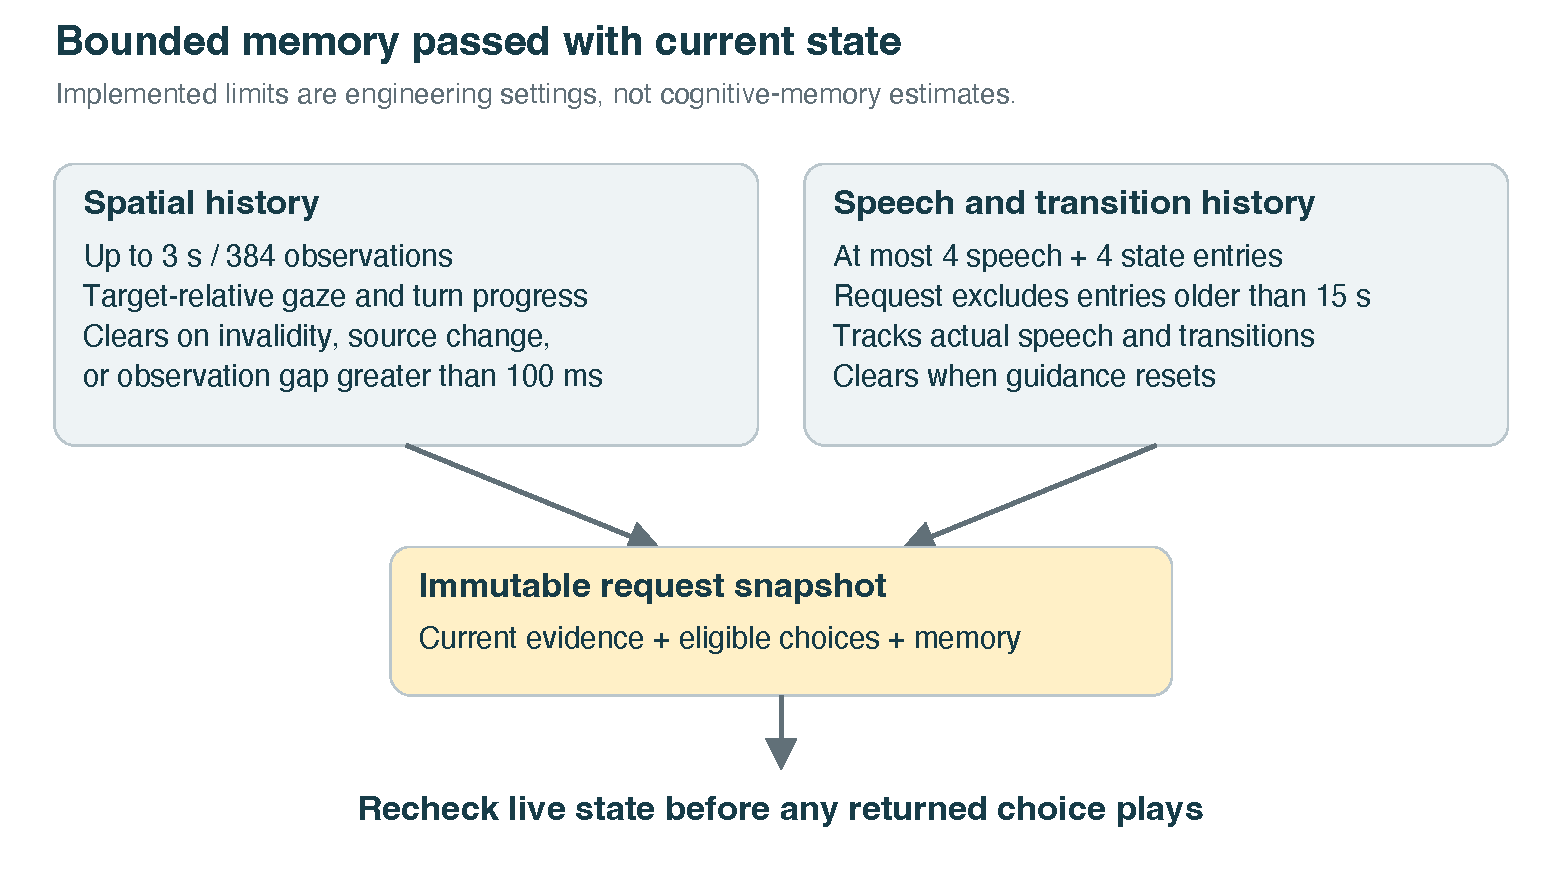
\includegraphics[width=\linewidth,alt={Spatial history and recent speech and state history are copied into a request and checked against current state before playback.}]{figures/bounded-memory.pdf}
\caption[Bounded spatial and speech memory]{Implemented memory limits and snapshot boundary. Spatial history and speech/state history have different retention and reset rules. A copied request preserves its original context, while playback still requires a fresh state check.}
\label{fig:bounded-memory}
\end{figure}


\section{Agent Decisions and Playback Control}
Jev selects from a constrained set of options rather than generating free-form instructions. Local geometry and state rules first filter the phrase library to candidates that are valid in the current situation. Each request to Jev contains a state snapshot, recent memory, playback status, and two to five eligible phrases. Jev then chooses the wording and whether to speak now or wait. Target definition and geometric reasoning remain local. Eligibility filtering and playback revalidation are intended to reduce spatially incorrect or stale guidance, but tracking error, imperfect geometry and software faults can still produce unhelpful instructions; recorded-sequence and headset checks remain necessary.

Because cloud responses arrive asynchronously, the participant's state may change before a decision returns. A local speech scheduler therefore revalidates each decision against the current state, evidence, pacing, and object intersections before playback, and discards decisions that are stale or conflict with the current situation. Qualified gaze and controller acknowledgments and eligible turn-progress milestones can use local handling and are played from prepared phrases without waiting for a new cloud decision, subject to the same checks. Each completed or interrupted utterance updates both the memory and the event log. Model latency, deferral, cancellation, fallback, and playback onset are logged separately to support delay attribution. When a trace lacks the required events, the cause remains unknown rather than inferred from the spoken phrase alone.

\begin{figure}[htbp]\centering
\IfFileExists{figures/voice-guidance-memory-architecture.pdf}{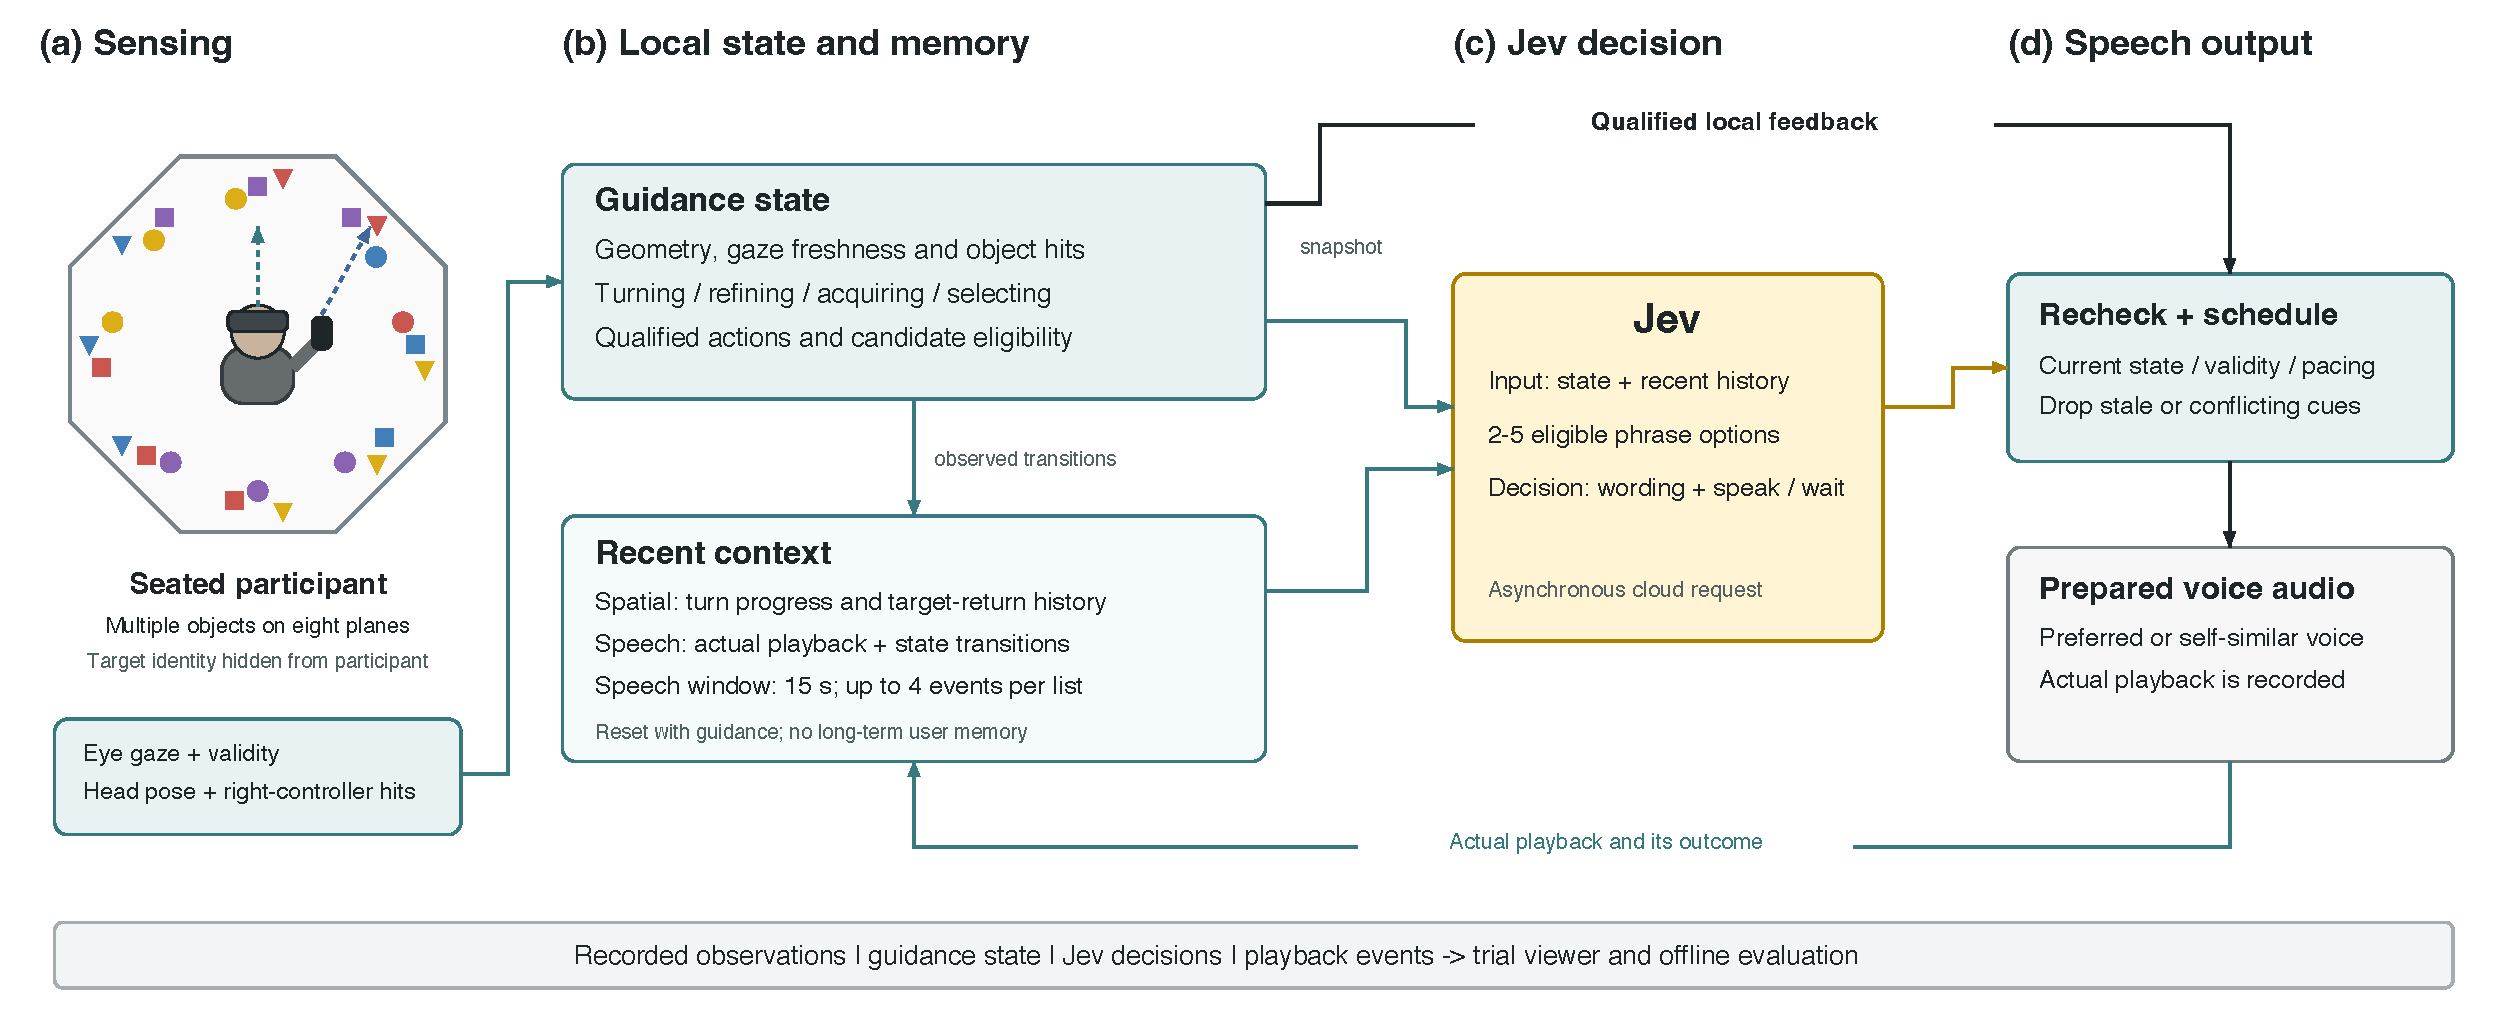
\includegraphics[width=\linewidth,alt={Gaze and controller sensing feed local state and memory, constrained Jev choices, a fresh playback check, and actual speech feedback.}]{figures/voice-guidance-memory-architecture.pdf}}{\fbox{\parbox{0.94\linewidth}{Gaze and controller observations $\rightarrow$ local state and bounded context $\rightarrow$ eligible choices for Jev $\rightarrow$ current-state recheck $\rightarrow$ prepared voice playback. Qualified local feedback also enters the recheck stage.}}}
\caption[Guidance architecture and playback control]{System architecture. (a) Gaze, head, and controller data are sensed. (b) A local state machine and short-term memory determine which guidance actions are valid. (c) Jev chooses wording and timing from eligible options. (d) The scheduler revalidates each cue against the current state before playback. Actual playback feeds back into memory. The scene inset is schematic and does not reflect stimulus count or any participant-visible target cue.}
\label{fig:architecture}
\end{figure}

\section{Voice Preparation and Telemetry}
All voice audio is pre-synthesized with ElevenLabs, which supplies both the catalog voice and the self-similar voice. To support the self-similar condition, each participant records the same standard passage in their usual speaking voice. Both conditions share the semantic phrase library, guidance policy, and playback routing. Voice condition is the intended manipulation; behavior-dependent wording, hint counts and synthesized acoustics need not be identical. The preparation pipeline checks wording and library readiness. Per-voice intelligibility, loudness and acoustic comparability still require pilot verification; automated checks do not establish perceptual equivalence. No pitch or spatial effects are applied to the self-similar voice. We log the provider, model, voice ID, library version, and synthesis settings.

The Trial Review application aligns gaze and controller state, guidance transitions, agent decisions, and playback events with trial geometry on a common timeline. Trial-level aggregates are stored separately from the raw gaze, motion, and event streams. Effective gaze sampling rate must be verified from distinct source timestamps on the tested headset build rather than inferred from the nominal specification or application polling rate. Similarly, the analysis will report ray intersections as gaze hits and do not label them as fixations unless a validated event classifier is applied.

\section{Trial Review Interface}
Figure~\ref{fig:trial-review-synthetic-demo} shows the standalone Trial Review application with its bundled synthetic demonstration. The scene and inspector share a timeline with speech, gaze, events, and decision tracks. The application also supports receiving headset records for live review; transfer and receipt times are separate from source event times, and late arrival must not be interpreted as delayed headset guidance. This capture illustrates the review interface only; it is not a participant recording or a performance result. In particular, the demonstration explicitly marks state history as missing and highlights as reconstructed. That distinction is useful when reviewing legacy records: the viewer should expose unavailable evidence rather than imply it was measured.

\begin{figure}[htbp]
\centering
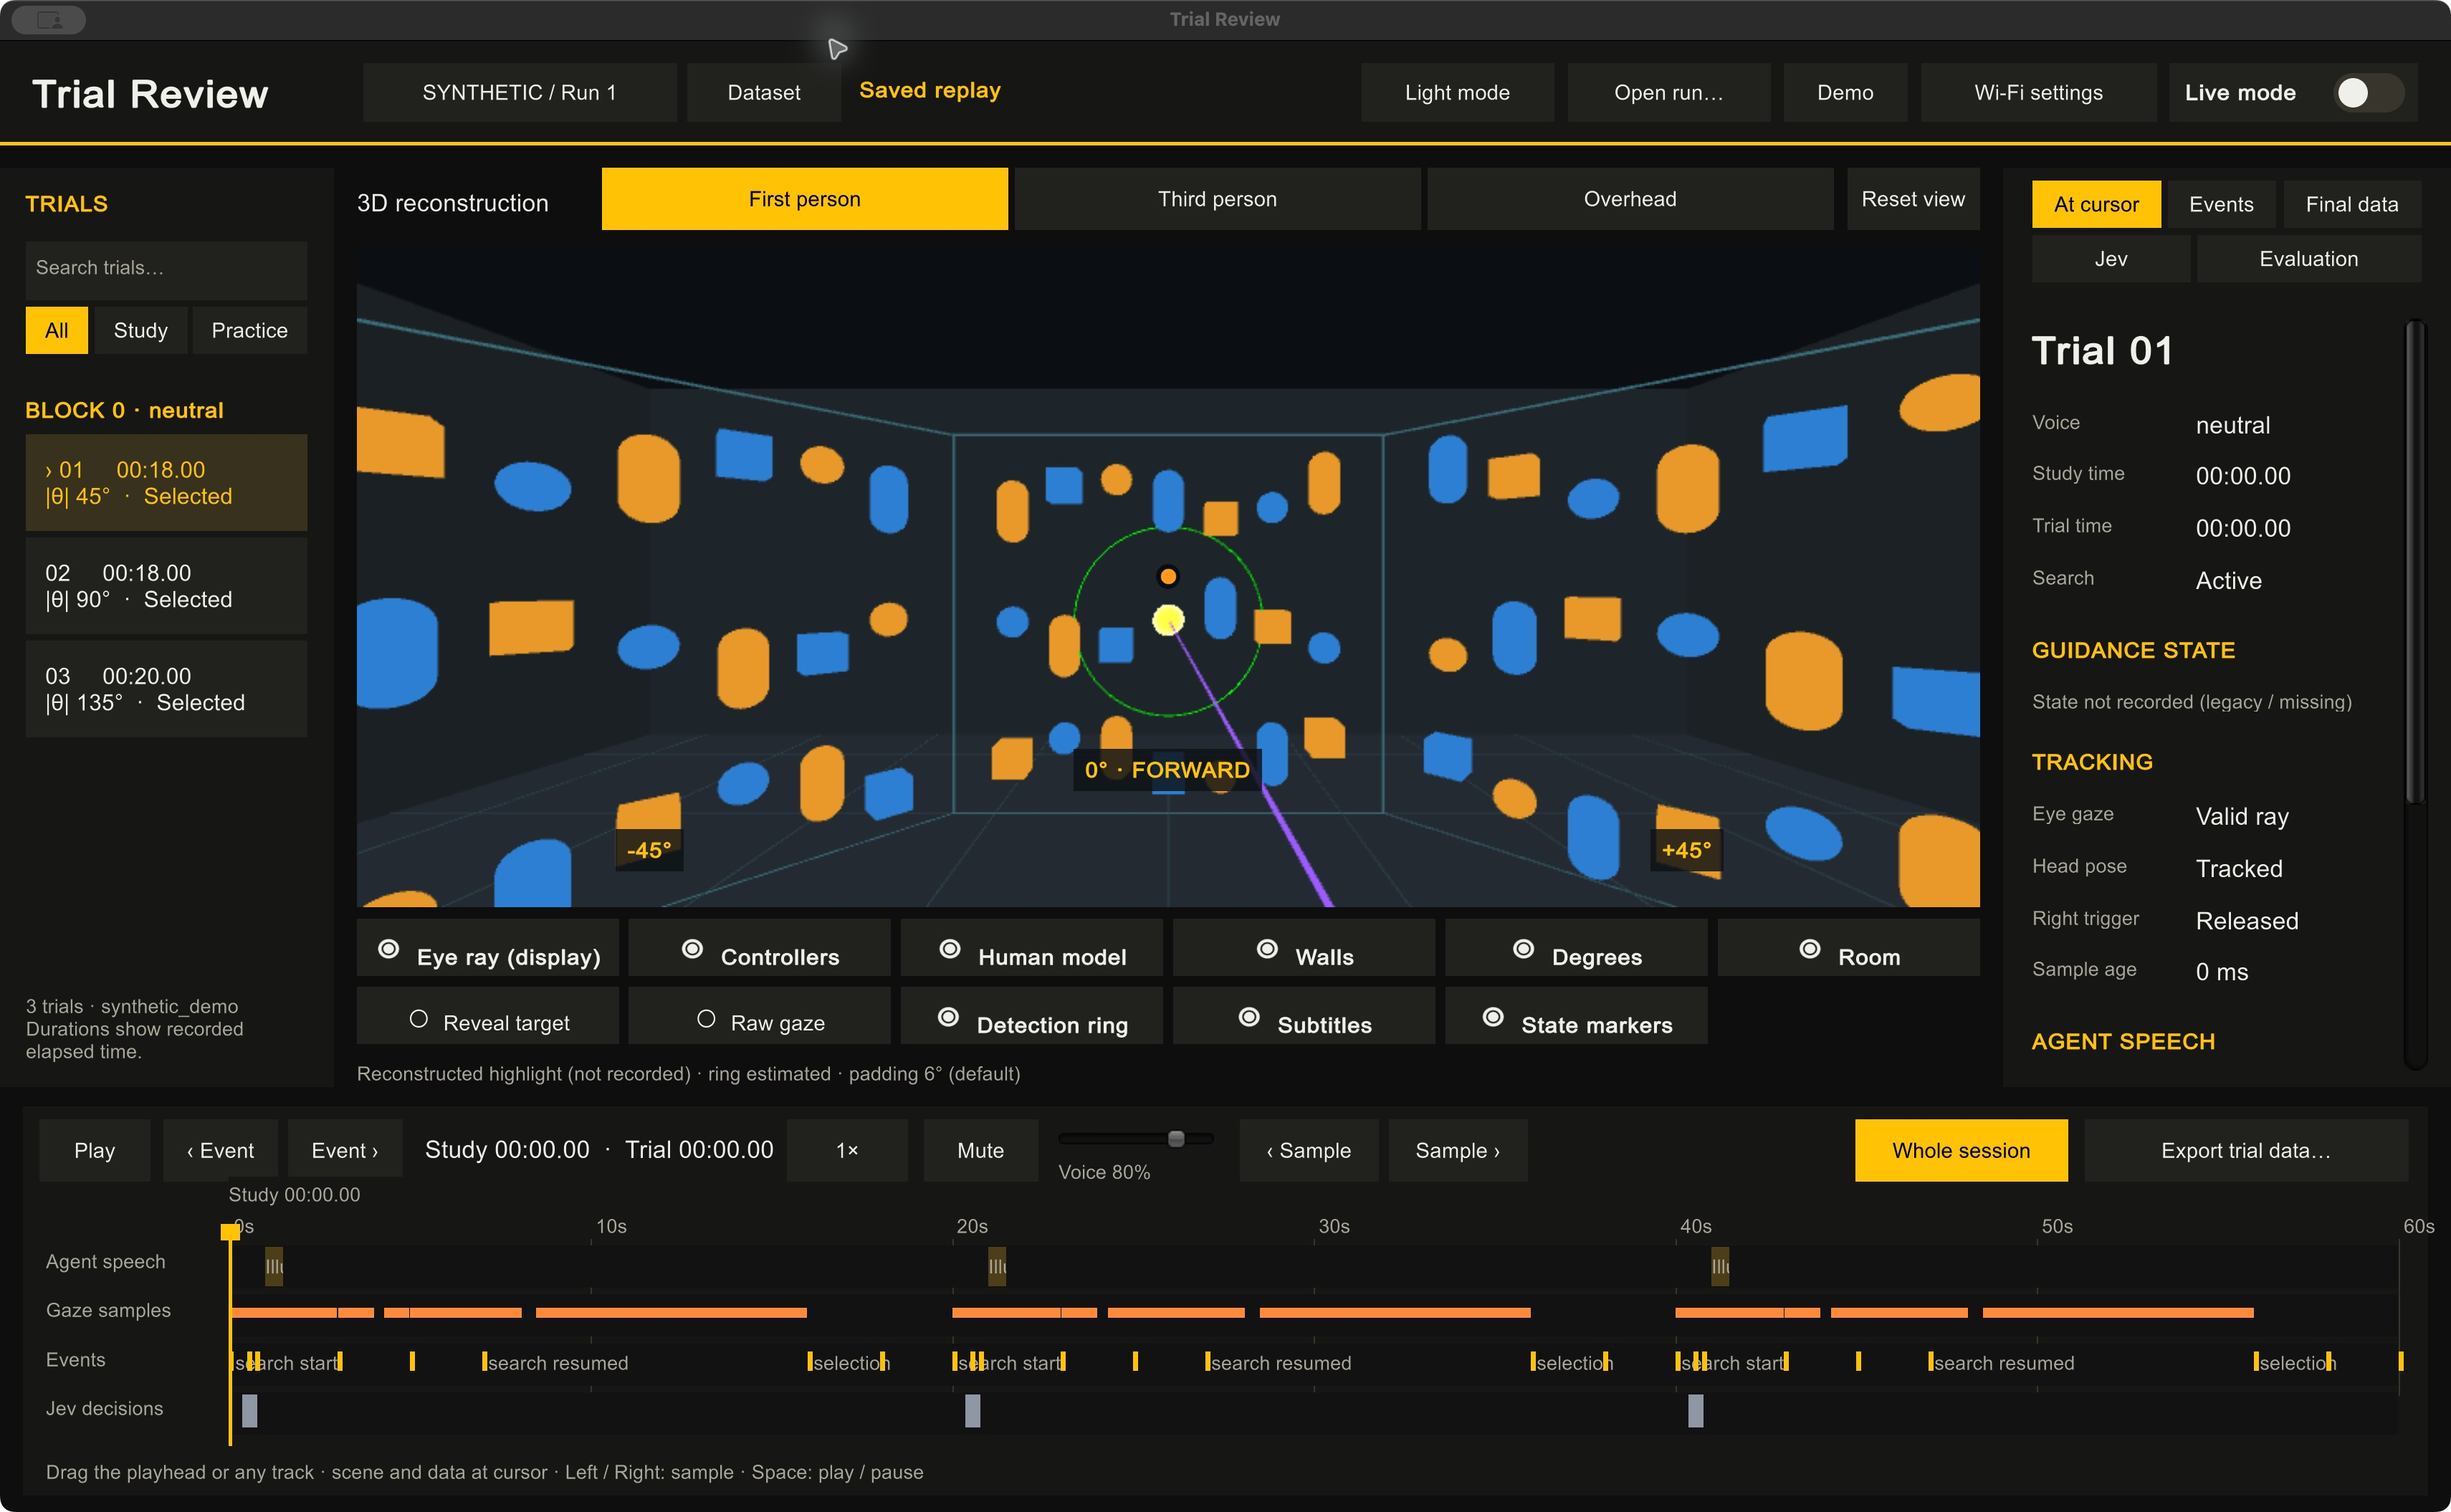
\includegraphics[width=\linewidth,alt={Trial Review application showing its explicitly synthetic three-trial demonstration, reconstructed scene, evidence inspector, and synchronized timeline.}]{figures/trial-review-synthetic-demo.png}
\caption[Trial Review interface with synthetic demonstration]{Actual application screenshot captured for this draft using the bundled SYNTHETIC / Run 1 demonstration. The central reconstruction, right-hand inspector, and timeline provide synchronized review. Missing state, estimated rings, and reconstructed highlights are labeled by the application. This is a visualization example, not headset video or empirical study data.}
\label{fig:trial-review-synthetic-demo}
\end{figure}


\section{Ownership and State Transitions}
The central guidance machine is a plain C\# object, while Unity MonoBehaviours connect it to tracked devices, scene objects, and audio. This separates deterministic state transitions from engine callbacks. The round manager owns readiness, trial onset, completion, pause intervals, and block progression. The guidance machine owns the interpretation of evidence during search. The speech scheduler owns pending requests, cancellation, and playback admission. These are coordinated responsibilities rather than a single global state variable controlling the whole application.

A state label is useful only when it is accompanied by its evidence. A refining state indicates that guidance has entered the target wall, but does not prove that the eyes intersect the target object. An acquired state can reflect qualified vicinity evidence, but does not mean a trigger selection occurred. The viewer therefore presents state transitions alongside gaze-hit, vicinity-candidate, controller-hit, and playback records. This makes it possible to inspect an apparent disagreement rather than assume the label is complete ground truth.

\begin{table}[htbp]
\centering\caption{Guidance responsibilities and evidence boundaries.}
\small\begin{tabularx}{\linewidth}{@{}p{0.22\linewidth}XX@{}}\toprule
Component & Owns & Does not establish \\\midrule
Observation adapters & Validity, poses, ray hits, source timing & Recognition or fixation \\
Guidance machine & Stage, eligible action, bounded history & Correct trigger selection or conscious recognition \\
Jev decision provider & Choice among eligible phrases; speak or wait & New target identity or unchecked geometry \\
Speech scheduler & Current-state check, pacing, cancellation, start & Acoustic arrival at the ear \\
Round manager & Readiness, reveal, selection, pauses and blocks & Independent validation of gaze accuracy \\
Trial Review & Reconstruction from saved evidence & Missing observations between recorded samples \\\bottomrule
\end{tabularx}
\end{table}

The usual path is turning toward a wall, refining within it, acquiring the target with gaze, and preparing to select. This is not a mandatory one-way chain. Participants can overshoot, revisit a wall, point before gaze qualifies, or lose tracking. The implemented state families represent these returns; release testing must verify them without repeatedly announcing a new arrival whenever the participant looks upward on the same wall. Invalid or stale evidence suspends new gaze-dependent decisions rather than treating the absence as a departure.

Figure~\ref{fig:guidance-states} summarizes the state families. The arrows show a common progression rather than compulsory transitions: correct right-trigger selection can complete an active trial without a preceding spoken gaze or pointing acknowledgment.

\begin{figure}[htbp]
\centering
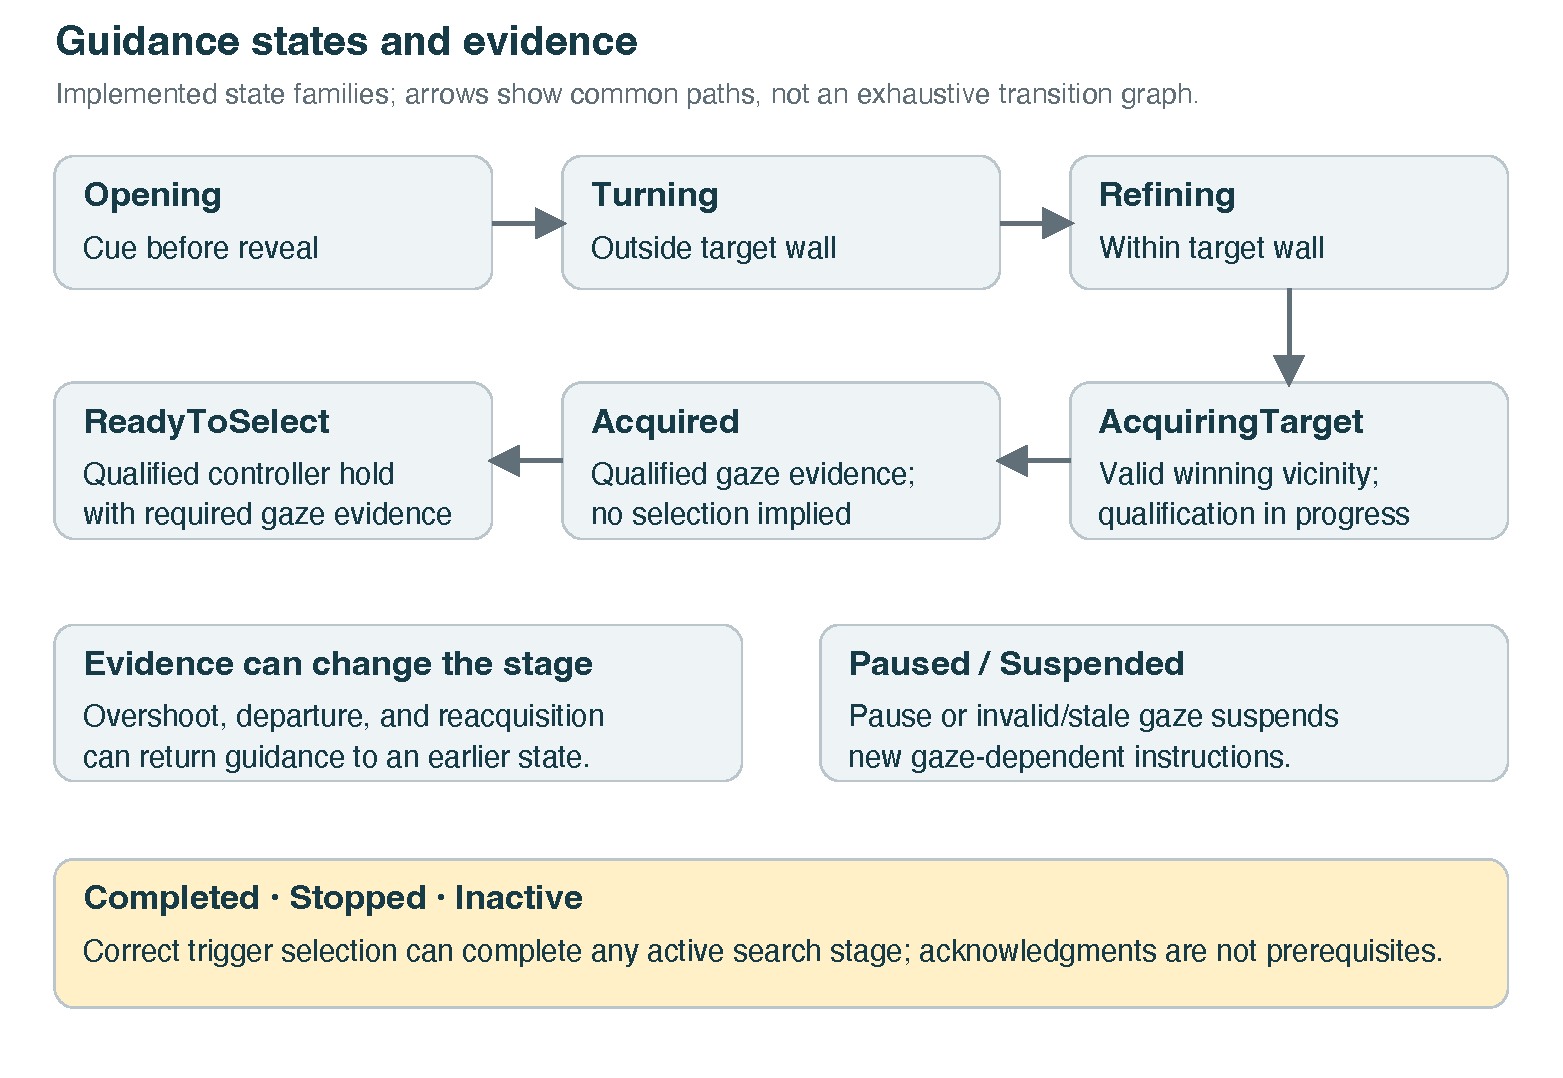
\includegraphics[width=\linewidth,alt={Common path from opening through turning and refinement to acquisition and readiness, with pause and suspension and independent trigger completion.}]{figures/guidance-states.pdf}
\caption[Guidance states and evidence-dependent transitions]{Implemented guidance state families. Turning, refining, acquisition, and readiness are evidence-dependent interpretations. Tracking loss, pauses, target departure, and reacquisition can change the path. Trial completion remains owned by the round manager.}
\label{fig:guidance-states}
\end{figure}


\section{A Worked Guidance Sequence}
Consider an illustrative target near the wall opposite the starting cross, with a rightward offset or the documented backward-turn tie rule. The opening cue may say that the object is to the right while objects remain hidden. Once search begins, progress cues can acknowledge continued rightward turning. On stable entry to the target wall, assistance can move to within-wall refinement, such as looking lower and slightly left. The reference for that refinement must be the recorded gaze geometry and local target relation, not a neighboring object's apparent screen position.

If the participant passes the target, recent spatial history can support a return cue. If the participant instead looks near the target long enough, a gaze acknowledgment becomes eligible. If the controller is already intersecting the target, away-directions are suppressed immediately. A qualified pointing acknowledgment can then identify controller evidence, and a right-trigger press can complete the trial. This example illustrates intended transitions; it is not a measured trajectory or evidence that all people follow this sequence.

\section{Asynchronous Decisions and Cancellation}
Each cloud request receives a snapshot, not a live reference to mutable state. The snapshot includes current evidence, relevant geometry, speech status, and bounded recent history. A response can become stale because the participant moves, tracking changes, the voice changes, a pause begins, or the trial ends. The scheduler checks those conditions again before playing the chosen clip. A valid answer to an old question is not necessarily a valid instruction now.

Prepared audio removes synthesis from the immediate hint path, but does not remove network latency from cloud choice. Time-sensitive qualified feedback can use local admission without waiting for another Jev decision. Ordinary hints can wait for phrasing choice within bounded scheduling rules. Interruption policy balances urgency against comprehensibility; finishing a short useful phrase may be preferable to cutting it at an awkward boundary. The documented implementation uses a 150-ms fade as a playback technique, not a guarantee of natural conversation.

Experimental policies that allow Jev broader action choice must be versioned separately from the participant policy. Replaying the same observations through multiple policies can compare decision latency and admissibility. It cannot show how a participant would have moved after hearing a different cue. The participant release will need one frozen policy and a manifest of thresholds, phrase library, Jev provider/model identifier, version and available sampling settings. Whether the provider sees voice-condition identifiers must be verified against the frozen payload; this draft does not assume condition-blind decisions. That audit will distinguish voice-related cancellation keys from information actually transmitted to the provider.
